\documentclass[a4paper,10pt]{report}
\usepackage[utf8]{inputenc}
\usepackage[francais]{babel}
\usepackage[top=1.5cm, bottom=1.5cm, left=1cm, right=1cm]{geometry}
\usepackage{graphicx}

% Title Page
\title{OMGL4 - Etape 4 : Développement de l'application}
\author{MAILLET Arnaud (chef de projet), VARGAS Christophe, ARDAUD Guillaume}


\begin{document}
\maketitle
\newpage
\null
\newpage
\tableofcontents
\newpage
\null
\newpage

\centering

%%%%%%%%%%%%%%%%%%%%%%%%%%%%%%%%%%%%%%%%%%%%%%%%%%%%%%%%%%%%%%%%%%%%%%%%%%%%%%%%%%%%%%%%%%%%%%%%%%%%%%%%%%%%%%%%%%%%%%%%%%%%%%%%%%%%%%%%%%%%%%%%%%%%%%%%%%%%%%%%%%%%%%%%%%%%%%%%%%%%%%%%%%%%%%%%%%%%%%%%%%%%%%%%%%%%%%%%%%%%%%%%%%%%%%%%%%%%%%%%%%%%%%%%%%%%%%%%%%%%%%%%%%%%%%%%%%%%%%%%%%%%%%%%%%%%%%%%%%%%%%%%%%%%%%%%%%

\chapter*{Nouvel ouvrage}
\addcontentsline{toc}{chapter}{Nouvel ouvrage}

Auteur : Christophe VARGAS
Relecteur : Arnaud MAILLET

\bigskip
\section*{Scenario principal}
\addcontentsline{toc}{section}{Scenario principal}
\begin{flushleft}
- La documentaliste demande l'enregistrement d'un nouvel ouvrage.\\
- Le Système demande le numéro ISBN.\\
- La documentaliste saisit l'ISBN.\\
- Le système recherche l'ouvrage.\\
- Le système demande les informations propres de l'ouvrage.\\
- La documentaliste saisit le titre, le nom de l'editeur, la date de parution.\\
- Le système crée l'ouvrage.\\
- Le système demande les auteurs de l'ouvrage.\\
- La documentaliste saisit les auteurs de l'ouvrage.\\
- Le système recherche les auteurs, les crée si ils n'éxistent pas et les lie à l'ouvrage.\\
- Le système demande les mots clés de l'ouvrage.\\
- La documentaliste saisit les mots clés de l'ouvrage.\\
- Le système recherche les mots clés et les lie à l'ouvrage.\\
- Le système confirme l'enregistrement du nouvel ouvrage.\\
\end{flushleft}

\bigskip

\section*{Diagramme de séquence haut niveau}
\addcontentsline{toc}{section}{Diagramme de séquence haut niveau}
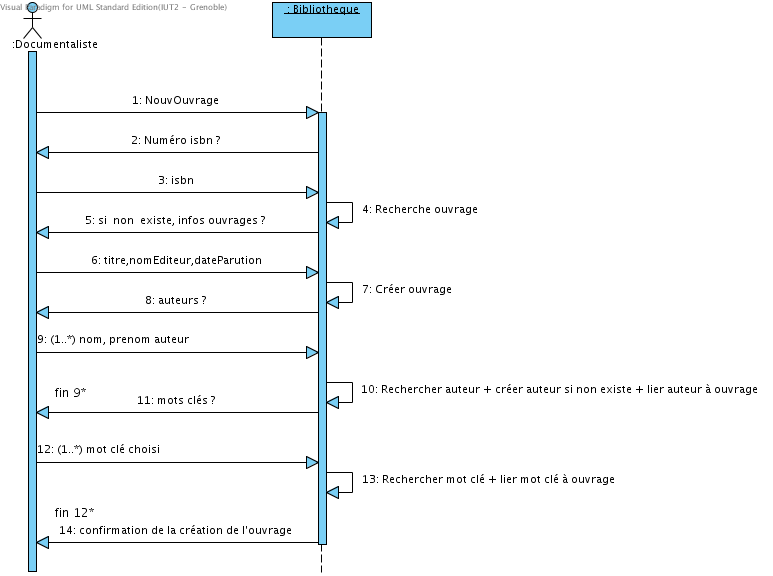
\includegraphics[height=90mm]{NouvOuvrageHautNiveau.png}

\newpage

\section*{Unité de présentation}
\addcontentsline{toc}{section}{Unité de présentation}
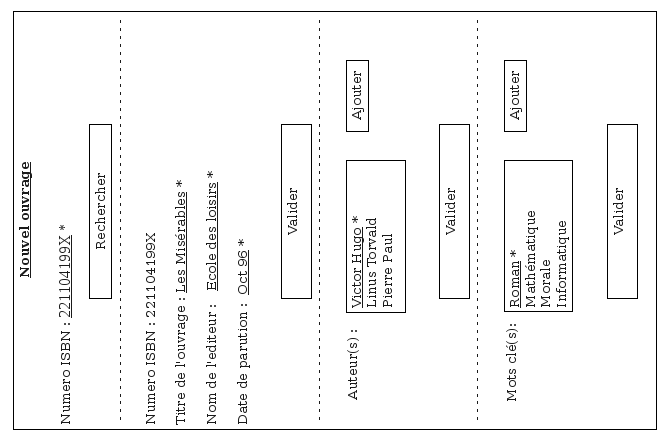
\includegraphics[height=70mm]{UpNouvOuvrage.png}

\section*{Diagramme de séquence détaillé MVC}
\addcontentsline{toc}{section}{Diagramme de séquence détaillé MVC}
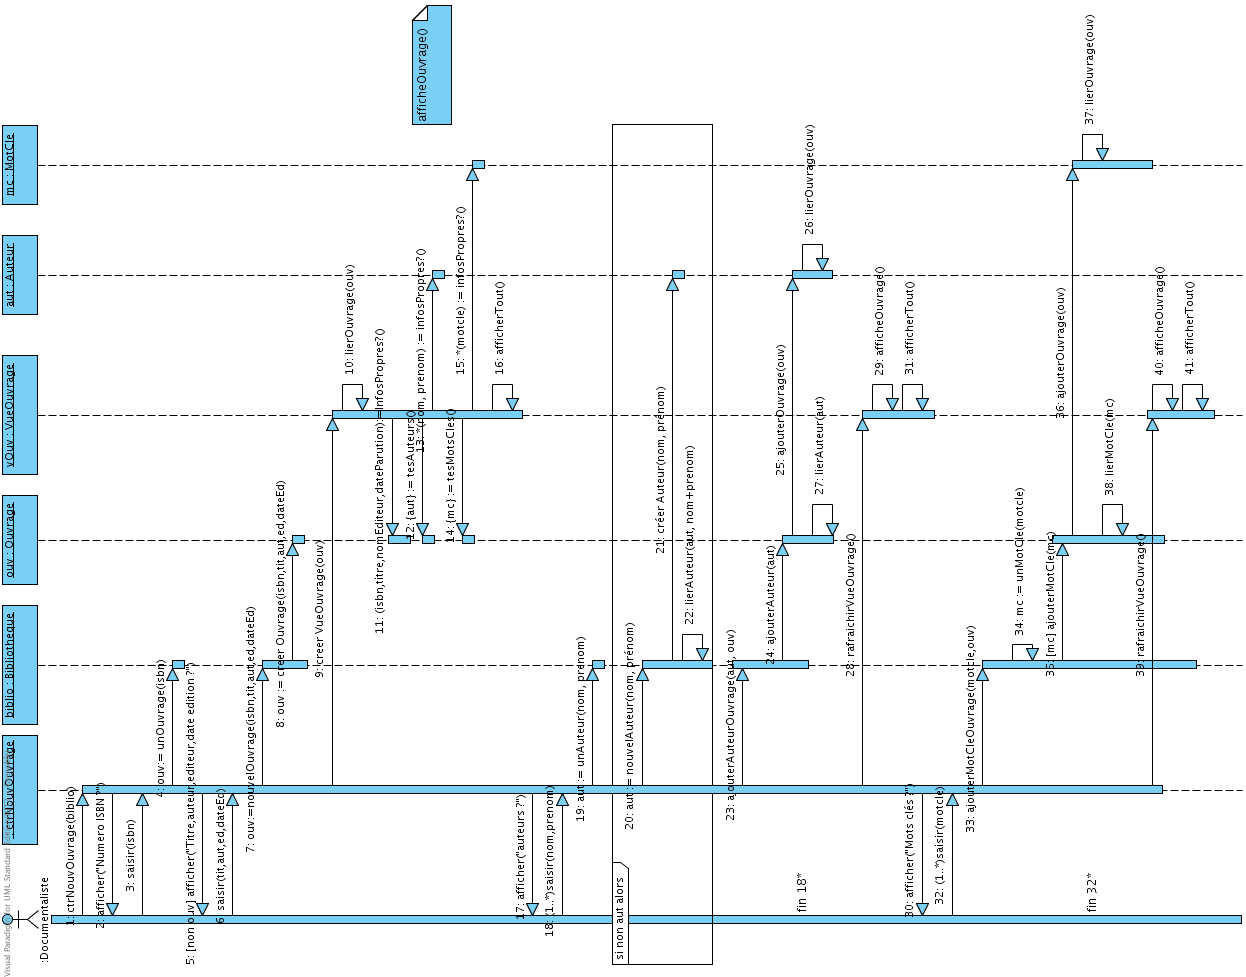
\includegraphics[height=145mm]{NouvOuvrageMVC.png}

\newpage

%%%%%%%%%%%%%%%%%%%%%%%%%%%%%%%%%%%%%%%%%%%%%%%%%%%%%%%%%%%%%%%%%%%%%%%%%%%%%%%%%%%%%%%%%%%%%%%%%%%%%%%%%%%%%%%%%%%%%%%%%%%%%%%%%%%%%%%%%%%%%%%%%%%%%%%%%%%%%%%%%%%%%%%%%%%%%%%%%%%%%%%%%%%%%%%%%%%%%%%%%%%%%%%%%%%%%%%%%%%%%%%%%%%%%%%%%%%%%%%%%%%%%%%%%%%%%%%%%%%%%%%%%%%%%%%%%%%%%%%%%%%%%%%%%%%%%%%%%%%%%%%%%%%%%%%%%%

\chapter*{Nouveau périodique}
\addcontentsline{toc}{chapter}{Nouveau périodique}

Auteur : Arnaud MAILLET
Relecteur : Christophe VARGAS

\bigskip
\section*{Scenario principal}
\addcontentsline{toc}{section}{Scenario principal}
\begin{flushleft}
-La documentaliste demande l'enregistrement d'un nouveau periodique.\\
-Le système demande le numéro ISSN et le nom du périodique.\\
-La documentaliste saisit le numéro ISSN et le nom du périodique.\\
-Le système créé le périodique.\\
-Le système confirme la création du périodique et affiche les informations propres du periodique.\\
\end{flushleft}

\bigskip

\section*{Diagramme de séquence haut niveau}
\addcontentsline{toc}{section}{Diagramme de séquence haut niveau}
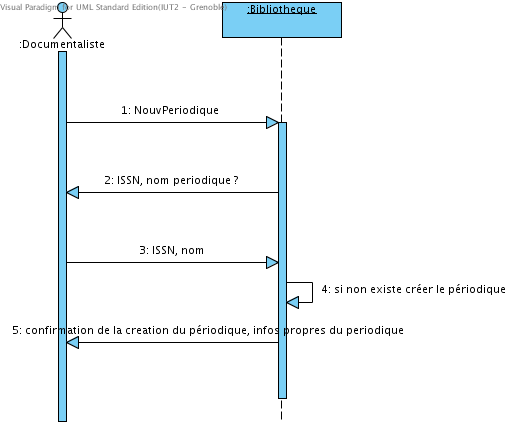
\includegraphics[height=90mm]{NouvPerHautNiveau.png}

\newpage

\section*{Unité de présentation}
\addcontentsline{toc}{section}{Unité de présentation}
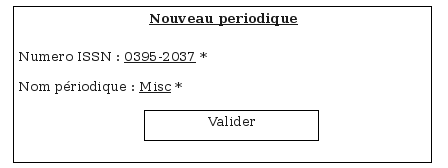
\includegraphics[height=70mm]{UpNouvPer.png}

\section*{Diagramme de séquence détaillé MVC}
\addcontentsline{toc}{section}{Diagramme de séquence détaillé MVC}
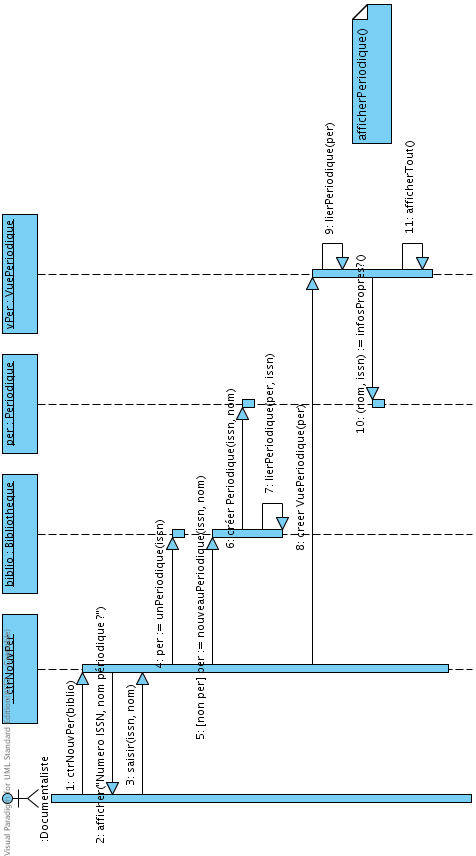
\includegraphics[height=150mm]{NouvPerMVC.png}

\newpage

%%%%%%%%%%%%%%%%%%%%%%%%%%%%%%%%%%%%%%%%%%%%%%%%%%%%%%%%%%%%%%%%%%%%%%%%%%%%%%%%%%%%%%%%%%%%%%%%%%%%%%%%%%%%%%%%%%%%%%%%%%%%%%%%%%%%%%%%%%%%%%%%%%%%%%%%%%%%%%%%%%%%%%%%%%%%%%%%%%%%%%%%%%%%%%%%%%%%%%%%%%%%%%%%%%%%%%%%%%%%%%%%%%%%%%%%%%%%%%%%%%%%%%%%%%%%%%%%%%%%%%%%%%%%%%%%%%%%%%%%%%%%%%%%%%%%%%%%%%%%%%%%%%%%%%%%%%

\chapter*{Nouveau numéro périodique}
\addcontentsline{toc}{chapter}{Nouveau numéro périodique}

Auteur : Arnaud MAILLET
Relecteur : Guillaume ARDAUD

\bigskip

\section*{Scenario principal}
\addcontentsline{toc}{section}{Scenario principal}
\begin{flushleft}
- La documentaliste demande l'enregistrement pour une nouvelle parution d'un périodique donné.\\
- Le système demande le numéro ISSN du périodique.\\
- La documentaliste saisit le numéro ISSN du périodique.\\
- Le système recherche le périodique dans le système informatique et affiche ses informations propres (nom périodique).\\
- Le système demande le numéro de parution de la nouvelle parution.\\
- La documentaliste saisit le numéro de parution de la nouvelle parution\\
- Le système créé la nouvelle parution et lie la nouvelle parution à son periodique.\\
- Pour tous les articles, le système demande les informations propres des articles de la parution (titre, page).\\
- La documentaliste saisit les informations propres des articles de la parution.\\
- le système crée l'article et lie l'article à la parution du periodique.\\
- Le système demande les auteurs de l'article.\\
- La documentaliste saisit les auteurs de l'article.\\
- Le système recherche les auteurs, les crée si ils n'éxistent pas et les lie à l'article.\\
- Le système demande les mots clés de l'article.\\
- La documentaliste saisit les mots clés de l'article.\\
- Le système recherche les mots clés et les lie à l'article.\\
- Le système confirme l'enregistrement de la nouvelle parution.\\
\end{flushleft}

\bigskip

\section*{Diagramme de séquence haut niveau}
\addcontentsline{toc}{section}{Diagramme de séquence haut niveau}
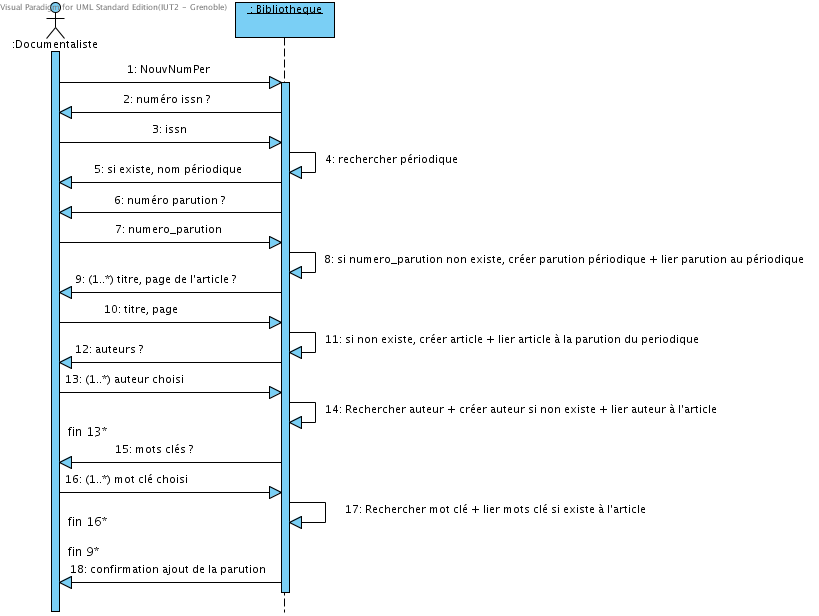
\includegraphics[height=90mm]{NouvNumPerHautNiveau.png}

\newpage

\section*{Unité de présentation}
\addcontentsline{toc}{section}{Unité de présentation}
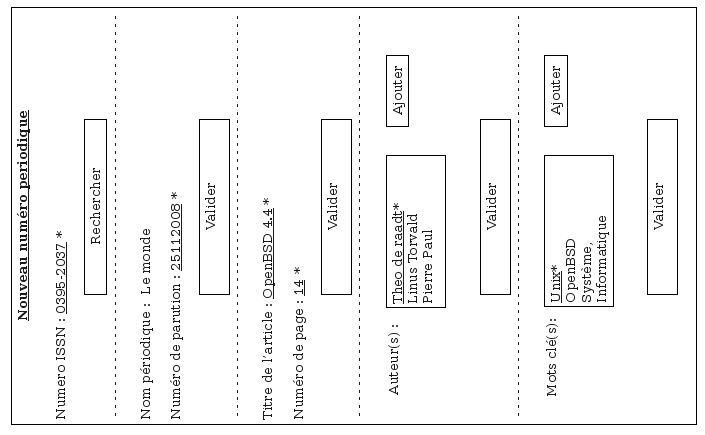
\includegraphics[height=70mm]{UpNouvNumPer.png}

\section*{Diagramme de séquence détaillé MVC}
\addcontentsline{toc}{section}{Diagramme de séquence détaillé MVC}
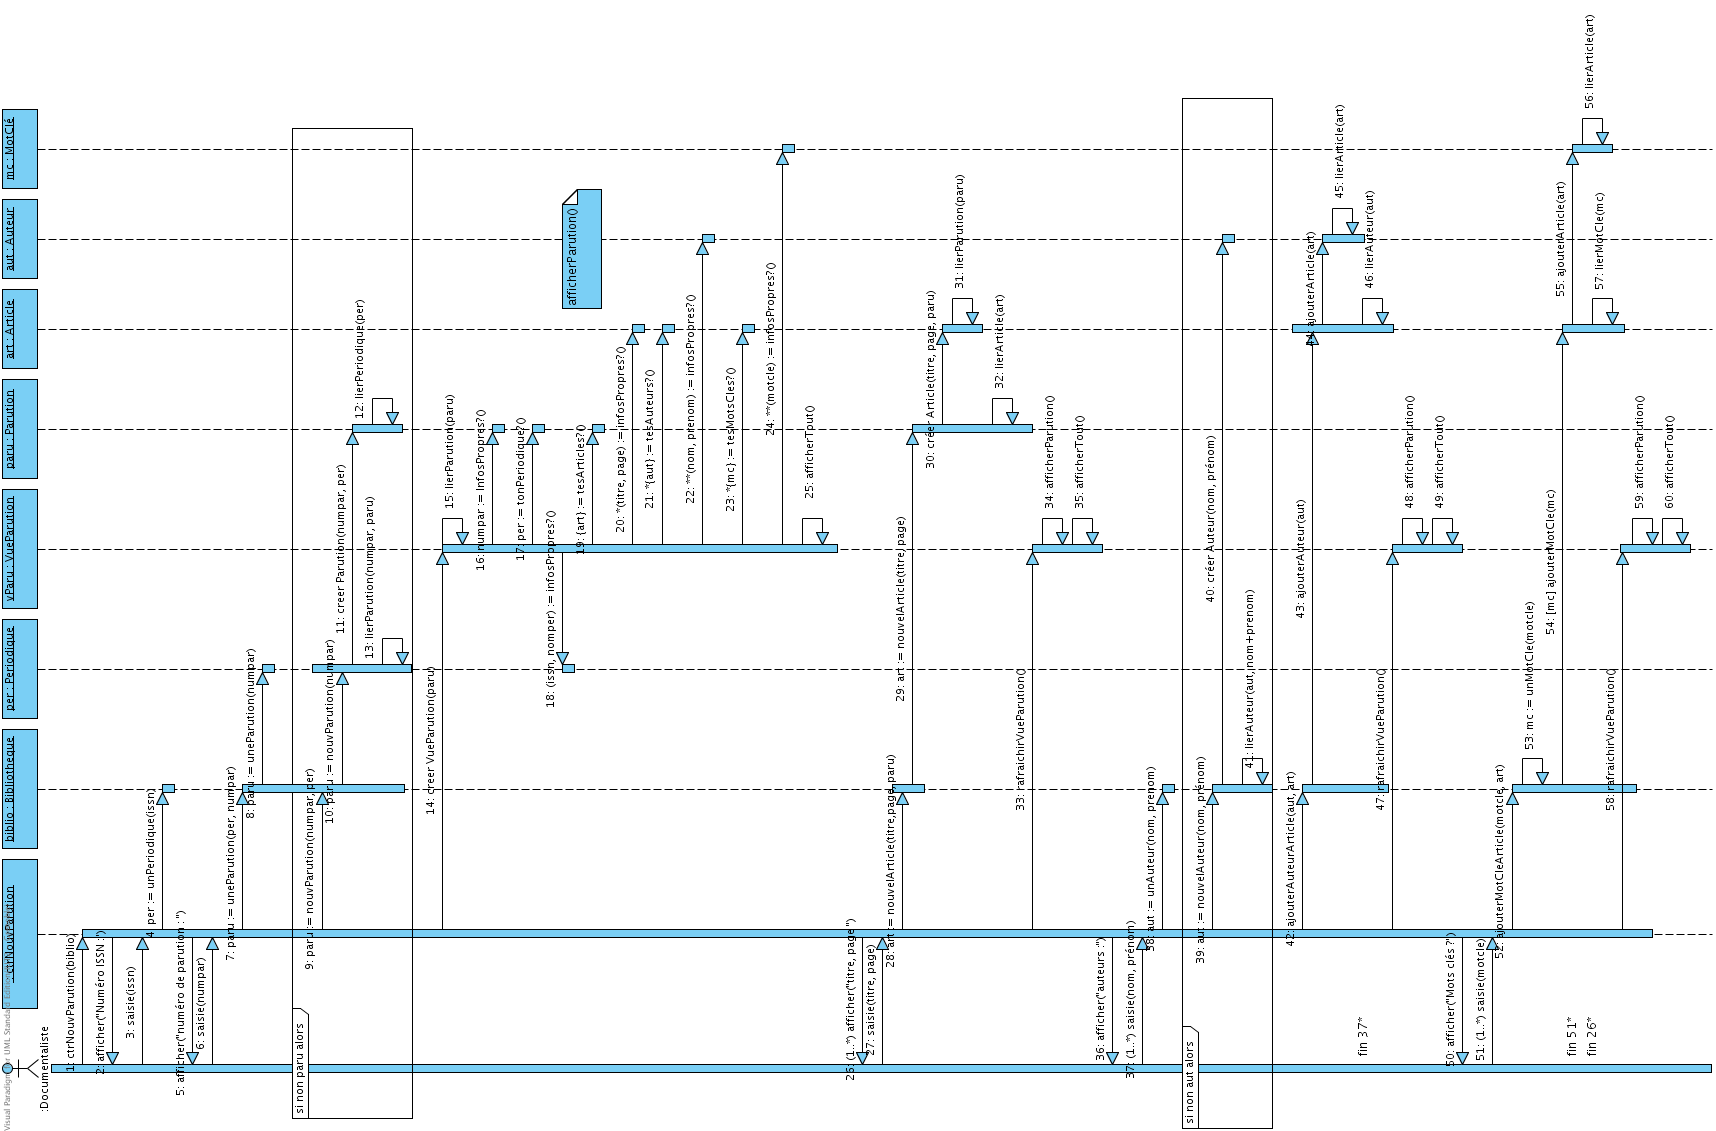
\includegraphics[height=120mm]{NouvNumPerMVC.png}

\newpage

%%%%%%%%%%%%%%%%%%%%%%%%%%%%%%%%%%%%%%%%%%%%%%%%%%%%%%%%%%%%%%%%%%%%%%%%%%%%%%%%%%%%%%%%%%%%%%%%%%%%%%%%%%%%%%%%%%%%%%%%%%%%%%%%%%%%%%%%%%%%%%%%%%%%%%%%%%%%%%%%%%%%%%%%%%%%%%%%%%%%%%%%%%%%%%%%%%%%%%%%%%%%%%%%%%%%%%%%%%%%%%%%%%%%%%%%%%%%%%%%%%%%%%%%%%%%%%%%%%%%%%%%%%%%%%%%%%%%%%%%%%%%%%%%%%%%%%%%%%%%%%%%%%%%%%%%%%

\chapter*{Consulter périodique (avec ses numéros)}
\addcontentsline{toc}{chapter}{Consulter périodique (avec ses numéros)}

Auteur : Christophe VARGAS
Relecteur : Arnaud MAILLET

\bigskip
\section*{Scenario principal}
\addcontentsline{toc}{section}{Scenario principal}
\begin{flushleft}
- La documentaliste demande la consultation d'un periodique.\\
- Le système demande le numéros ISSN.\\
- La documentaliste saisit l'ISSN.\\
- Le système recherche Le periodique, ses parutions et les articles des parutions.\\
- Le système affiche le periodique, ses parutions et les articles des parutions.\\
\end{flushleft}

\bigskip

\section*{Diagramme de séquence haut niveau}
\addcontentsline{toc}{section}{Diagramme de séquence haut niveau}
\bigskip
\bigskip
\bigskip
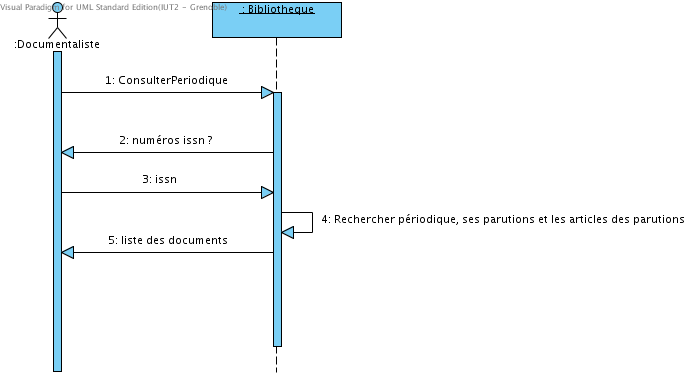
\includegraphics[height=90mm]{ConsPeriodiqueHautNiveau.png}

\newpage

\section*{Unité de présentation}
\addcontentsline{toc}{section}{Unité de présentation}
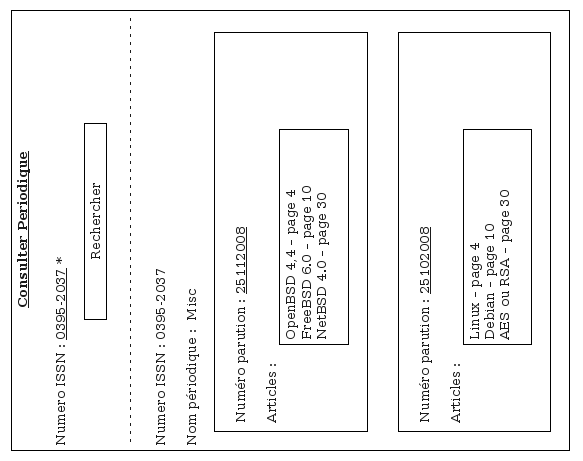
\includegraphics[height=70mm]{UpConsPeriodique.png}

\section*{Diagramme de séquence détaillé MVC}
\addcontentsline{toc}{section}{Diagramme de séquence détaillé MVC}
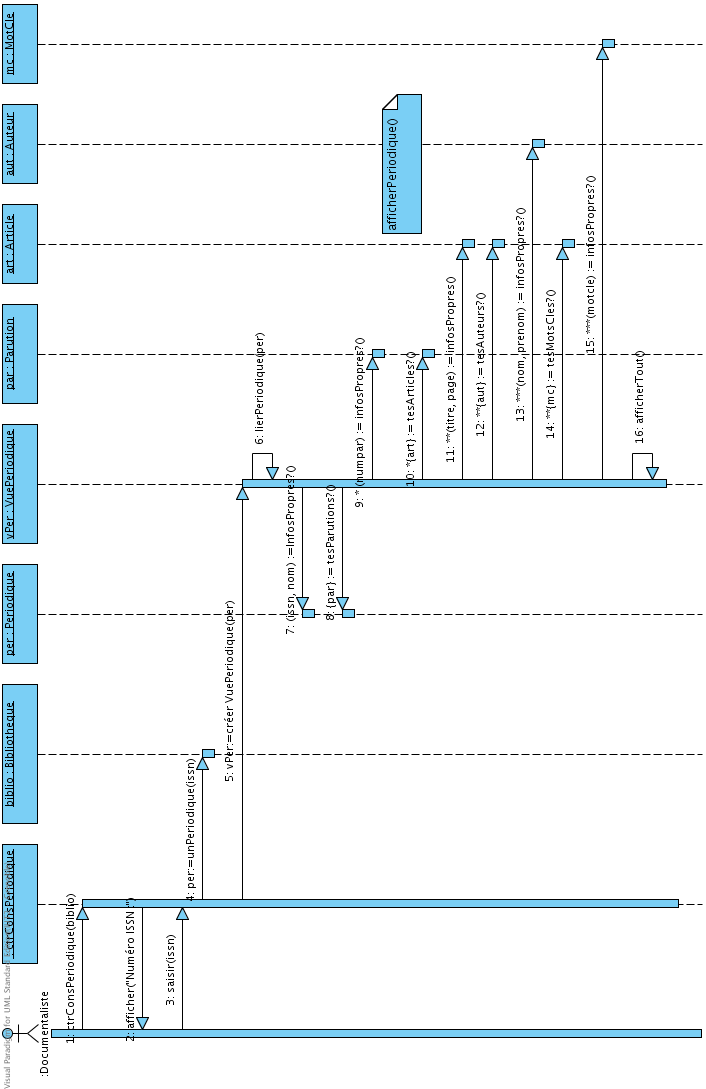
\includegraphics[height=150mm]{ConsPeriodiqueMVC.png}

\newpage

%%%%%%%%%%%%%%%%%%%%%%%%%%%%%%%%%%%%%%%%%%%%%%%%%%%%%%%%%%%%%%%%%%%%%%%%%%%%%%%%%%%%%%%%%%%%%%%%%%%%%%%%%%%%%%%%%%%%%%%%%%%%%%%%%%%%%%%%%%%%%%%%%%%%%%%%%%%%%%%%%%%%%%%%%%%%%%%%%%%%%%%%%%%%%%%%%%%%%%%%%%%%%%%%%%%%%%%%%%%%%%%%%%%%%%%%%%%%%%%%%%%%%%%%%%%%%%%%%%%%%%%%%%%%%%%%%%%%%%%%%%%%%%%%%%%%%%%%%%%%%%%%%%%%%%%%%%

\chapter*{Recherche par auteur}
\addcontentsline{toc}{chapter}{Recherche par auteur}

Auteur : Arnaud MAILLET
Relecteur : Christophe VARGAS

\bigskip
\section*{Scenario principal}
\addcontentsline{toc}{section}{Scenario principal}
\begin{flushleft}
- La documentaliste demande la recherche par auteur.\\
- Le système demande l'auteur.\\
- La documentaliste saisit le nom et le prénom de l'auteur.\\
- Le système recherche l'auteur et ensuite le système recherche les ouvrages et les articles correspondant à cet auteur.\\
- Le système affiche la liste des documents.\\
\end{flushleft}

\bigskip

\section*{Diagramme de séquence haut niveau}
\addcontentsline{toc}{section}{Diagramme de séquence haut niveau}
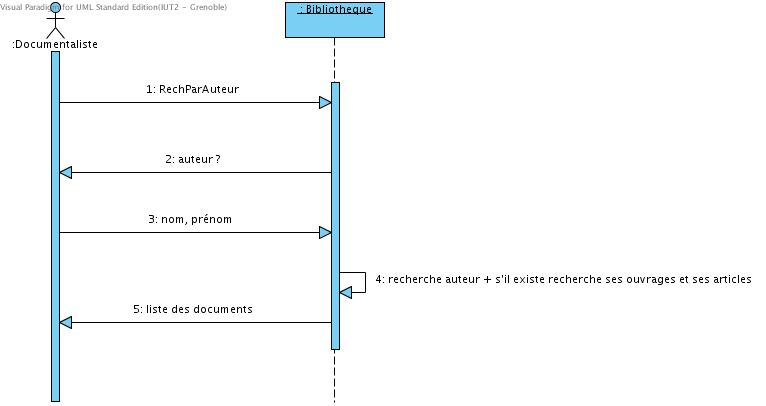
\includegraphics[height=90mm]{RechParAuteurHautNiveau.png}

\newpage

\section*{Unité de présentation}
\addcontentsline{toc}{section}{Unité de présentation}
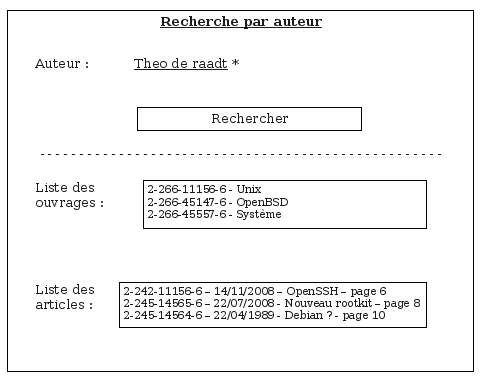
\includegraphics[height=70mm]{UpRechParAuteur.png}

\section*{Diagramme de séquence détaillé MVC}
\addcontentsline{toc}{section}{Diagramme de séquence détaillé MVC}
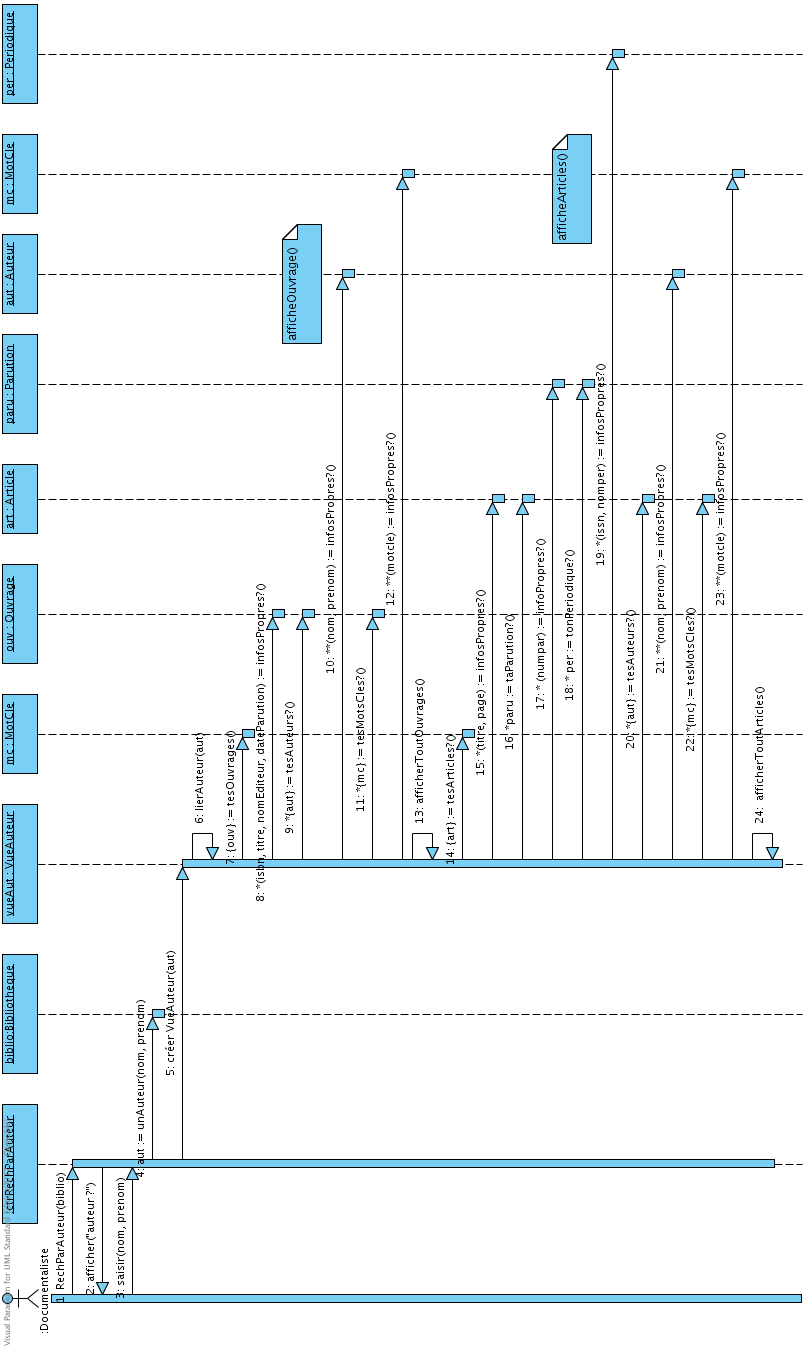
\includegraphics[height=150mm]{RechParAuteurMVC.png}

\newpage

%%%%%%%%%%%%%%%%%%%%%%%%%%%%%%%%%%%%%%%%%%%%%%%%%%%%%%%%%%%%%%%%%%%%%%%%%%%%%%%%%%%%%%%%%%%%%%%%%%%%%%%%%%%%%%%%%%%%%%%%%%%%%%%%%%%%%%%%%%%%%%%%%%%%%%%%%%%%%%%%%%%%%%%%%%%%%%%%%%%%%%%%%%%%%%%%%%%%%%%%%%%%%%%%%%%%%%%%%%%%%%%%%%%%%%%%%%%%%%%%%%%%%%%%%%%%%%%%%%%%%%%%%%%%%%%%%%%%%%%%%%%%%%%%%%%%%%%%%%%%%%%%%%%%%%%%%%

\chapter*{Recherche par mot clé}
\addcontentsline{toc}{chapter}{Recherche par mot clé}

Auteur : Arnaud MAILLET
Relecteur : Guillaume ARDAUD

\bigskip
\section*{Scenario principal}
\addcontentsline{toc}{section}{Scenario principal}
\begin{flushleft}
- La documentaliste demande la recherche par mot clé.\\
- Le système demande le mot clé.\\
- La documentaliste saisit le mot clé.\\
- Le système recherche le mots clé et ensuite le système recherche les ouvrages et les articles correspondant à ce mot clé.\\
- Le système affiche la liste des documents.\\
\end{flushleft}

\bigskip

\section*{Diagramme de séquence haut niveau}
\addcontentsline{toc}{section}{Diagramme de séquence haut niveau}
\bigskip
\bigskip
\bigskip
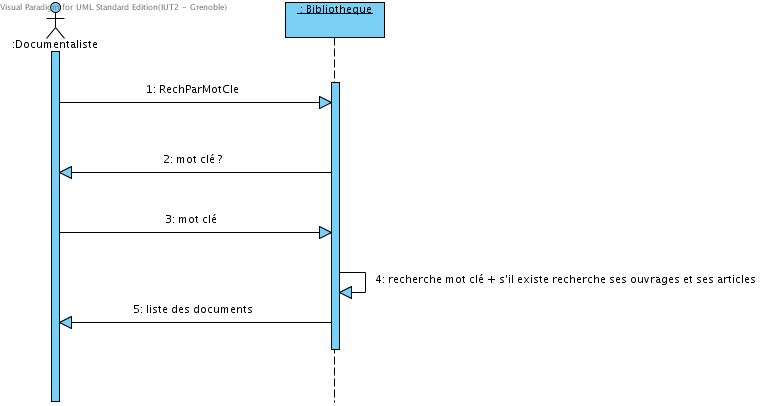
\includegraphics[height=100mm]{RechParMotCleHautNiveau.png}

\newpage

\section*{Unité de présentation}
\addcontentsline{toc}{section}{Unité de présentation}
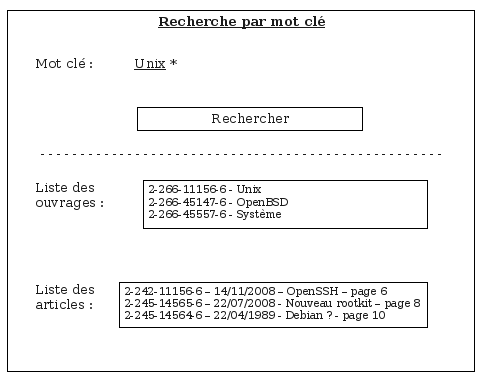
\includegraphics[height=70mm]{UpRechParMotCle.png}

\section*{Diagramme de séquence détaillé MVC}
\addcontentsline{toc}{section}{Diagramme de séquence détaillé MVC}
\bigskip
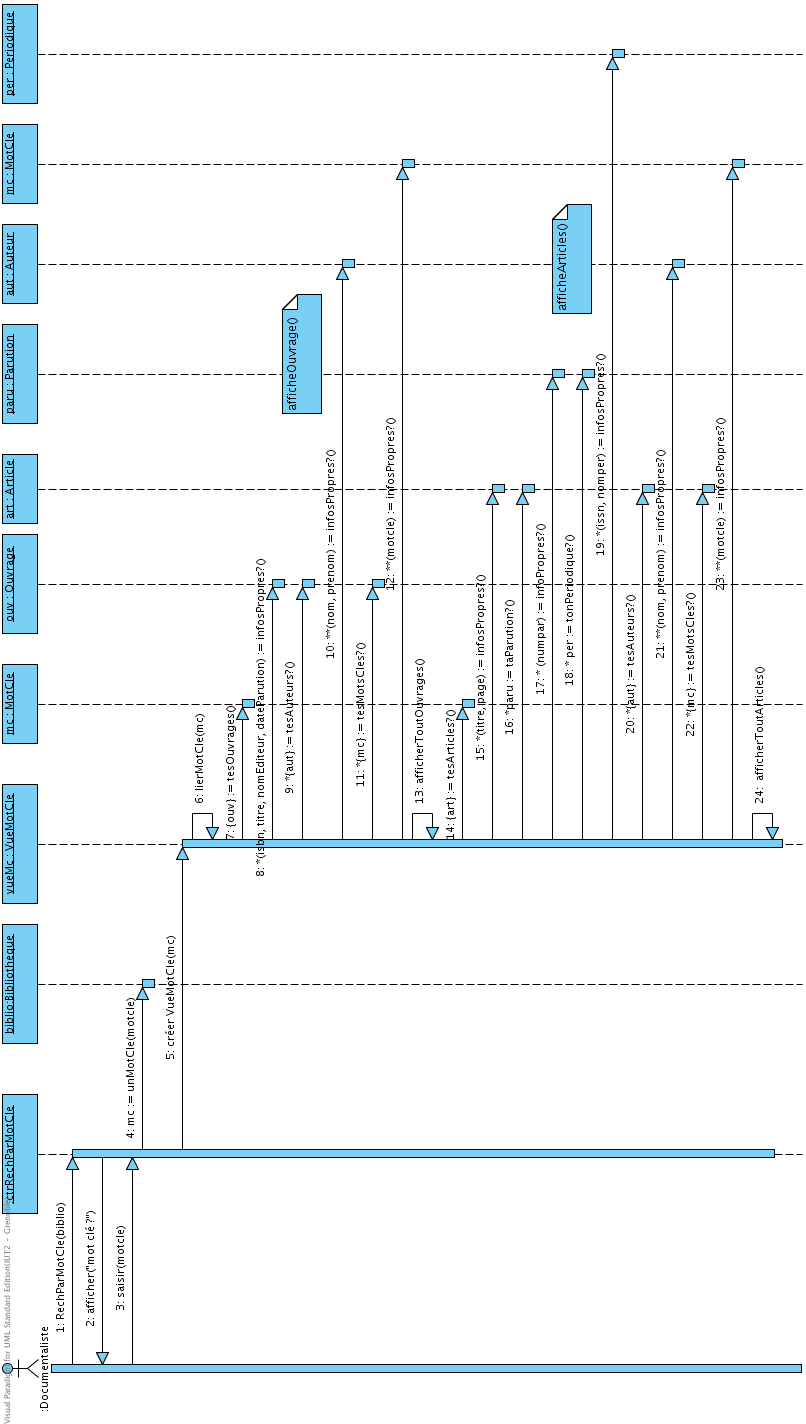
\includegraphics[height=165mm]{RechParMotCleMVC.png}

\newpage

%%%%%%%%%%%%%%%%%%%%%%%%%%%%%%%%%%%%%%%%%%%%%%%%%%%%%%%%%%%%%%%%%%%%%%%%%%%%%%%%%%%%%%%%%%%%%%%%%%%%%%%%%%%%%%%%%%%%%%%%%%%%%%%%%%%%%%%%%%%%%%%%%%%%%%%%%%%%%%%%%%%%%%%%%%%%%%%%%%%%%%%%%%%%%%%%%%%%%%%%%%%%%%%%%%%%%%%%%%%%%%%%%%%%%%%%%%%%%%%%%%%%%%%%%%%%%%%%%%%%%%%%%%%%%%%%%%%%%%%%%%%%%%%%%%%%%%%%%%%%%%%%%%%%%%%%%%

\chapter*{Emprunt exemplaire}
\addcontentsline{toc}{chapter}{Emprunt exemplaire}

Auteur : Arnaud MAILLET
Relecteur : Christophe VARGAS

\bigskip
\section*{Scenario principal}
\addcontentsline{toc}{section}{Scenario principal}
\begin{flushleft}
- La documentaliste demande l'emprunt d'un exemplaire.\\
- Le système demande le numéro du lecteur.\\
- La documentaliste saisit le numéro du lecteur.\\
- Le système recherche le lecteur et verifie si il peut emprunter.\\
- Le système demande le numéro ISSN de l'ouvrage et le numéro de l'exemplaire.\\
- La documentaliste saisit le numéro ISSN de l'ouvrage et le numéro de l'exemplaire.\\
- Le système recherche l'exemplaire et vérifie qu'il est empruntable. Le système créé l'emprunt, lie le lecteur et l'exemplaire à l'emprunt et il rend l'exemplaire "emprunté".\\
- Le système confirme l'emprunt de l'exemplaire.\\
\end{flushleft}

\bigskip

\section*{Diagramme de séquence haut niveau}
\addcontentsline{toc}{section}{Diagramme de séquence haut niveau}
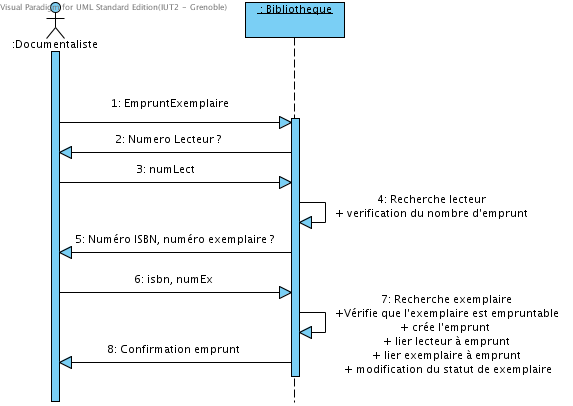
\includegraphics[height=90mm]{EmpruntExemplaireHautNiveau.png}

\newpage

\section*{Unité de présentation}
\addcontentsline{toc}{section}{Unité de présentation}
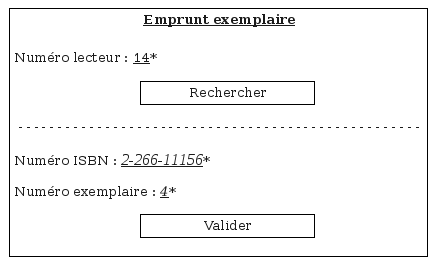
\includegraphics[height=70mm]{UpEmpruntExemplaire.png}

\section*{Diagramme de séquence détaillé MVC}
\addcontentsline{toc}{section}{Diagramme de séquence détaillé MVC}
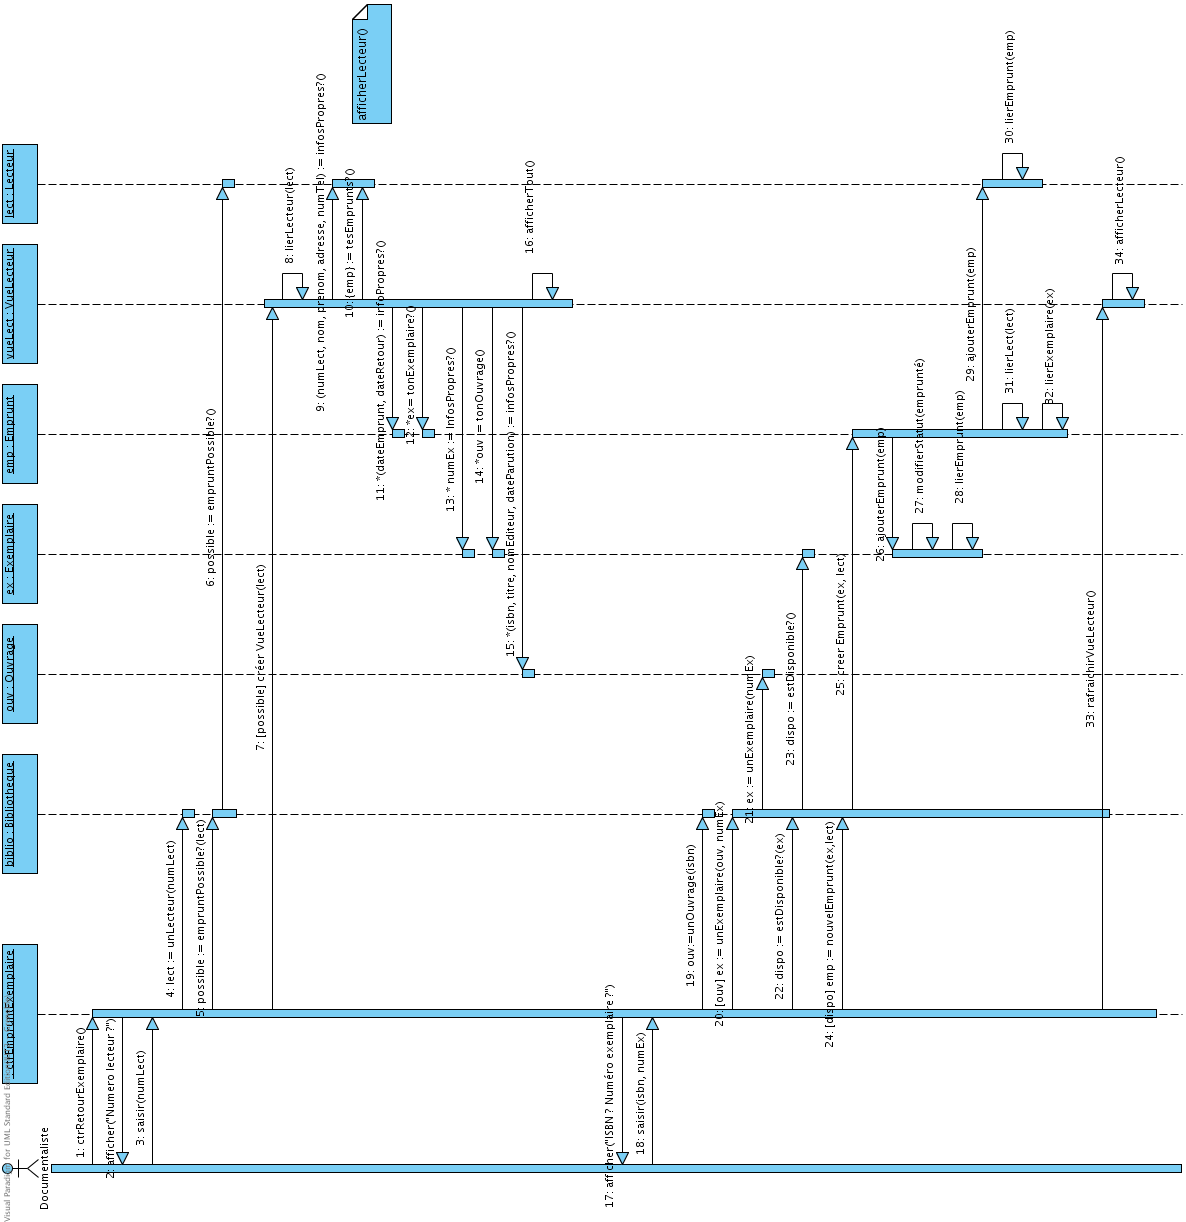
\includegraphics[height=150mm]{EmpruntExemplaireMVC.png}

\newpage

%%%%%%%%%%%%%%%%%%%%%%%%%%%%%%%%%%%%%%%%%%%%%%%%%%%%%%%%%%%%%%%%%%%%%%%%%%%%%%%%%%%%%%%%%%%%%%%%%%%%%%%%%%%%%%%%%%%%%%%%%%%%%%%%%%%%%%%%%%%%%%%%%%%%%%%%%%%%%%%%%%%%%%%%%%%%%%%%%%%%%%%%%%%%%%%%%%%%%%%%%%%%%%%%%%%%%%%%%%%%%%%%%%%%%%%%%%%%%%%%%%%%%%%%%%%%%%%%%%%%%%%%%%%%%%%%%%%%%%%%%%%%%%%%%%%%%%%%%%%%%%%%%%%%%%%%%%

\chapter*{Retour exemplaire}
\addcontentsline{toc}{chapter}{Retour exemplaire}

Auteur : Arnaud MAILLET
Relecteur : Christophe VARGAS

\bigskip
\section*{Scenario principal}
\addcontentsline{toc}{section}{Scenario principal}
\begin{flushleft}
- La documentaliste demande le retour d'un exemplaire.\\
- Le système demande le numéro du lecteur.\\
- La documentaliste saisit le numéro du lecteur.\\
- Le système recherche le lecteur.\\
- Le système demande le numéro ISSN de l'ouvrage et le numéro de l'exemplaire.\\
- La documentaliste saisit le numéro ISSN de l'ouvrage et le numéro de l'exemplaire.\\
- Le système recherche l'exemplaire puis son emprunt, s'ils existent le système enleve le lecteur et l'exemplaire de l'emprunt. Il rend l'exemplaire empruntable et détruit l'emprunt.\\
- Le système confirme le retour de l'exemplaire.\\
\end{flushleft}

\bigskip

\section*{Diagramme de séquence haut niveau}
\bigskip
\bigskip
\addcontentsline{toc}{section}{Diagramme de séquence haut niveau}
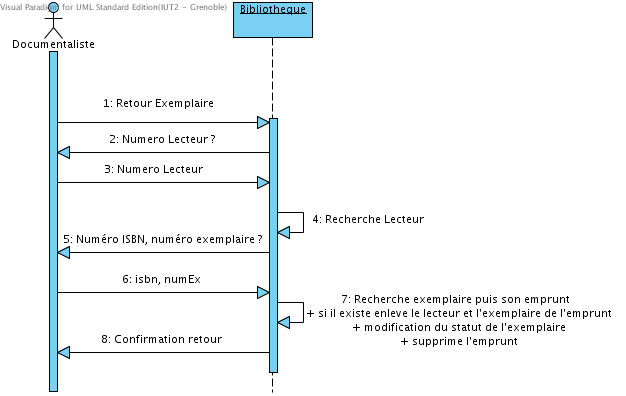
\includegraphics[height=90mm]{RetourExemplaireHautNiveau.png}

\newpage

\section*{Unité de présentation}
\addcontentsline{toc}{section}{Unité de présentation}
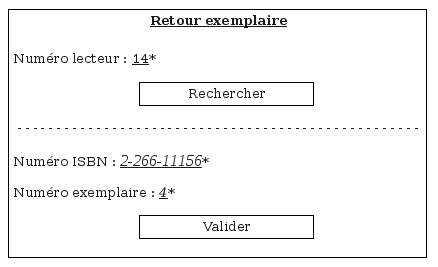
\includegraphics[height=70mm]{UpRetourExemplaire.png}

\section*{Diagramme de séquence détaillé MVC}
\bigskip
\bigskip
\addcontentsline{toc}{section}{Diagramme de séquence détaillé MVC}
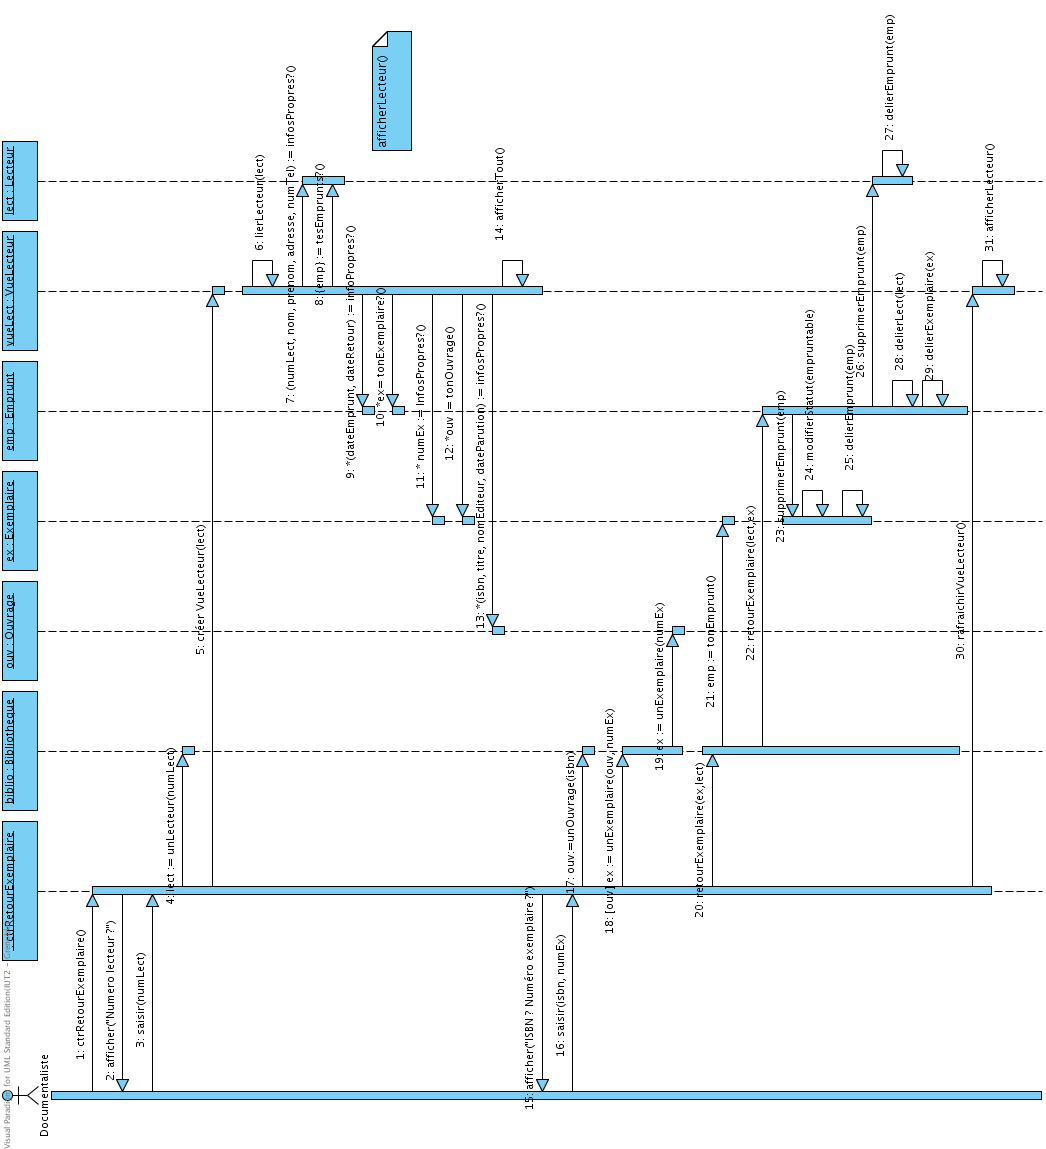
\includegraphics[height=150mm]{RetourExemplaireMVC.png}

\newpage

\chapter*{Autres}
\addcontentsline{toc}{chapter}{Autres}

Auteur : Arnaud MAILLET
Relecteur : Christophe VARGAS

\bigskip

\section*{Diagramme de classes généralisé}
\addcontentsline{toc}{section}{Diagramme de classes généralisé}
\bigskip
\bigskip
\begin{center}
voir ci contre
\end{center}
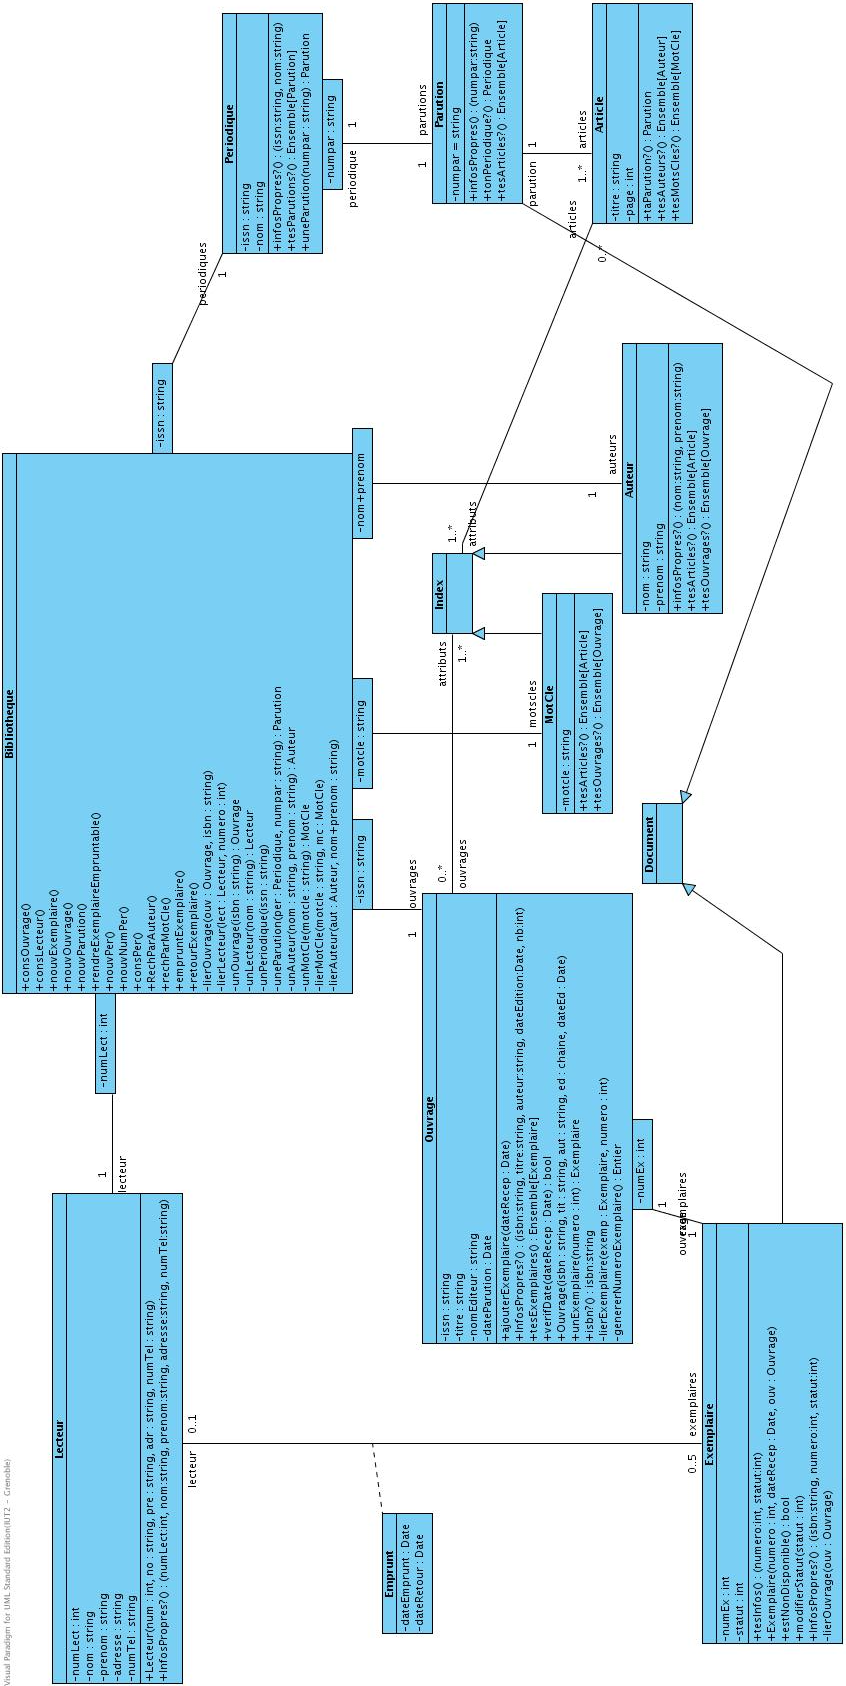
\includegraphics[height=260mm]{diagrammeDeClasseGeneralise.png}
\newpage
\section*{Description de la base et du jeux d'essai}
\addcontentsline{toc}{section}{Description de la base et du jeux d'essai}
\bigskip
\bigskip
\begin{flushleft}
Lecteur 1 :
\begin{itemize}
 \item MAILLET
 \item Arnaud
 \item 5 rue honoré de balzac Echirolles 38130
 \item 19
\end{itemize}
\bigskip
Lecteur 2 :
\begin{itemize}
 \item VARGAS
 \item Christophe
 \item 33 rue du suc St Julien 63320 Montaigut-le-blanc
 \item 20
\end{itemize}
\bigskip
Lecteur 3 : ( à ajouter )
\begin{itemize}
 \item ARDAUD
 \item Guillaume
 \item 3 rue Victor Hugo 38000 Grenoble
 \item 19
\end{itemize}
\bigskip
\bigskip
Ouvrage 1 : 
\begin{itemize}
 \item 978-2-7460-4617-7
 \item Scripts Shell sous Linux
 \item Baranger Jean-Marc - Shomaker Théo
 \item Eni
 \item informatique - sciences
 \item 13/11/2008
 \item Exemplaires :
	\begin{enumerate}
		\item 01/01/2009 - non disponible - Emprunté par Lecteur 1
		\item 02/01/2009 - non disponible - Emprunté par Lecteur 1
		\item 03/01/2009 - non disponible - Emprunté par Lecteur 1
		\item 04/01/2009 - en consultation
		\item 05/01/2009 - non disponible ( Changer statut )
	\end{enumerate}
\end{itemize}
\bigskip
Ouvrage 2 :
\begin{itemize}
 \item 978-2-212-11601-4
 \item Programmation système en C sous Linux
 \item Blaess Christophe
 \item Eyrolles
 \item informatique - sciences
 \item 03/03/2005
 \item Exemplaires :
	\begin{enumerate}
		\item 01/01/2009 - non disponible - Emprunté par Lecteur 1
		\item 02/01/2009 - empruntable ( à emprunter par Lecteur 1 )
		\item 03/01/2009 - empruntable ( à emprunter par Lecteur 1 )
		\item 04/01/2009 - en consultation
		\item 05/01/2009 - non disponible
	\end{enumerate}
\end{itemize}
\bigskip
Ouvrage 3 : ( à ajouter )
\begin{itemize}
 \item 978-2-212-12326-5
 \item Programmer en Java
 \item Claude Delannoy
 \item Eyrolles
 \item informatique - sciences
 \item 03/04/2008
\end{itemize}
\bigskip
\bigskip
\newpage
Periodique 1 :
\begin{itemize}
 \item 1244-4901
 \item Misc
 \item Parutions :
	\begin{itemize}
		\item Janvier / Février 2009
		\item Articles :
		\begin{itemize}
			\item La cybercriminalité aujourd’hui - 18 - Jean-Raymond Abrial -Informatique
			\item Extorsion par dénis de service - 34 - Pierre Bézier - Informatique
			\item Blanchiment d’argent sur Internet - 52 - Dan Bricklin - Informatique ( à ajouter )
		\end{itemize}
		\item Novembre/Décembre 2008 ( à ajouter ) 
		\item Articles :
		\begin{itemize}
			\item Conflit russo-géorgien et guerre de l’information - 4 - Bob Carr - Informatique ( à ajouter )
			\item Le très haut débit – Un challenge pour la sécurité - 29 - Alain Colmerauer - Informatique ( à ajouter )
		\end{itemize}
	\end{itemize}
\end{itemize}
 
\end{flushleft}

\end{document}